\section{LDR (Low Dynamic Range)}

\subsection{Descripción}

El filtro LDR modifica las zonas mas brillantes de la imagen, realzando o disminuyendo su brillo según el parametro alpha sea positivo o negativo.

Formalmente,
$$
    O^k_{i,j} = ldr^k_{i,j} = I^k_{i,j} + \alpha \frac{sumargb_{i,j}}{max} I^k_{i,j}
    \qquad \forall k \in \{r,g,b\},\; i,j \in \mathbb{N} \;\text{tq}\; 2 \le i < w - 2 \:\land\: 2 \le j < h - 2
$$
donde
\
$$ sumargb_{i,j} = \sum_{-2 \le u,v \le 2,\; k \in \{r,g,b\}} I^k_{i+u, j+v} $$
$$ max = 5 * 5 * 255 * 3 * 255 $$
\
y los $O^k_{i,j}$ no definidos mantienen su valor inicial.
$\\$

Como para procesar cada pixel necesitamos el valor de sus vecinos no podremos aplicar el filtro en los bordes de la imagen, por lo que quedan sin modificar.

Inicialmente se nos ocurrieron tres algoritmos para realizar el filtro:

\begin{enumerate}

\item Iterar sobre cada pixel. Si está en el borde copiarlo directamente, sino calcular su sumargb leyendo los 25 vecinos y guardar los valores correspondientes al pixel.

    Este método tiene una implementación trivial, pero un rendimiento pésimo debido a que debe acceder 26 veces a memoria para procesar cada pixel y realiza cálculos repetidos de las sumas de cada pixel.

\item Recorrer cada pixel de la imagen calculando la suma de sus canales $r,g,b$, y guardar el resultado en una matriz auxiliar.

    Luego recorrer nuevamente los pixeles no-borde y realizar la función usando los valores precalculados.

    Con este método evitamos repetir los cálculos de la suma de los canales de cada pixel, pero implica usar $\mathcal{O}(ancho * altura)$ memoria adicional (como la suma de tres bytes siempre entra en un word y no necesitamos copiar el alpha, la matriz tendrá la mitad del tamaño de la imagen). Además agrega el overhead de los accesos a memoria y ocupa espacio extra en la caché.

\item Recorrer cada pixel excepto los de las filas inferiores y superiores calculando $$\sum_{-2 \le v \le 2,\; k \in \{r,g,b\}} I^k_{i, j+v}$$ esto es, la suma de su columna $\pm 2$.
    Mantener siempre los últimos cuatro resultados en memoria y al calcular el nuevo valor realizar la suma entre ellos y usarlos para procesar el pixel $(i-2,j)$, si no es un borde.

    De esta forma logramos evitar algunos cálculos repetidos pero mantenemos el uso de memoria extra constante.

\end{enumerate}

De estos algoritmos decidimos implementar la primer opción en C, ya que es el metodo trivial contra el que queremos comparar.

Para nuestras implementaciones en assembler utilizamos el tercer método, ya que consideramos que era el que ofrecía mas potencial para paralelizar con instrucciones SSE.

\subsection{Implementaciones}

\subsubsection{C}

El código de C es bastante simple, recorre cada pixel de la imagen y:

\begin{itemize}
    \item Si es un borde, lo copiamos directamente.

    \item Si no es un borde, recorremos los 25 vecinos acumulando la suma de sus componentes, y así obtenemos sumargb.
        Luego calculamos el resto de la fórmula y guardamos el valor final.
\end{itemize}

\subsubsection{Asm - SSE}

Para implementar el algoritmo $(3)$ recorremos la imagen procesando de a 4 píxeles, manteniendo la suma de las 4 ultimas columnas y calculando 4 nuevas en cada loop.


\begin{table}[h]
\centering
\asm{memoria}
\begin{tabular}{l|c|c|c|c|c|c|c|c|l}
 & \multicolumn{1}{l|}{}      & \multicolumn{1}{l|}{}       & \multicolumn{1}{l|}{}       & \multicolumn{1}{l|}{}
 & \multicolumn{1}{l|}{}      & \multicolumn{1}{l|}{}       & \multicolumn{1}{l|}{}       & \multicolumn{1}{l|}{}       &  \\ \hline

 & \cellcolor[HTML]{76E6A3}$I_{i-2,j+2}$ & \cellcolor[HTML]{98D0AE}$I_{i-1,j+2}$ & \cellcolor[HTML]{76E6A3}$I_{i  ,j+2}$ & \cellcolor[HTML]{98D0AE}$I_{i+1,j+2}$
 & \cellcolor[HTML]{FFBB78}$I_{i+2,j+2}$ & \cellcolor[HTML]{FF9D3E}$I_{i+3,j+2}$ & \cellcolor[HTML]{FFBB78}$I_{i+4,j+2}$ & \cellcolor[HTML]{FF9D3E}$I_{i+5,j+2}$ &  \\ \hline

 & \cellcolor[HTML]{76E6A3}$I_{i-2,j+1}$ & \cellcolor[HTML]{98D0AE}$I_{i-1,j+1}$ & \cellcolor[HTML]{76E6A3}$I_{i  ,j+1}$ & \cellcolor[HTML]{98D0AE}$I_{i+1,j+1}$
 & \cellcolor[HTML]{FFBB78}$I_{i+2,j+1}$ & \cellcolor[HTML]{FF9D3E}$I_{i+3,j+1}$ & \cellcolor[HTML]{FFBB78}$I_{i+4,j+1}$ & \cellcolor[HTML]{FF9D3E}$I_{i+5,j+1}$ &  \\ \hline

 & \cellcolor[HTML]{76E6A3}$I_{i-2,j  }$ & \cellcolor[HTML]{98D0AE}$I_{i-1,j  }$ & \cellcolor[HTML]{B1B1B1}$I_{i  ,j  }$ & \cellcolor[HTML]{B1B1B1}$I_{i+1,j  }$
 & \cellcolor[HTML]{B1B1B1}$I_{i+2,j  }$ & \cellcolor[HTML]{B1B1B1}$I_{i+3,j  }$ & \cellcolor[HTML]{FFBB78}$I_{i+4,j  }$ & \cellcolor[HTML]{FF9D3E}$I_{i+5,j  }$ &  \\ \hline

 & \cellcolor[HTML]{76E6A3}$I_{i-2,j-1}$ & \cellcolor[HTML]{98D0AE}$I_{i-1,j-1}$ & \cellcolor[HTML]{76E6A3}$I_{i  ,j-1}$ & \cellcolor[HTML]{98D0AE}$I_{i+1,j-1}$
 & \cellcolor[HTML]{FFBB78}$I_{i+2,j-1}$ & \cellcolor[HTML]{FF9D3E}$I_{i+3,j-1}$ & \cellcolor[HTML]{FFBB78}$I_{i+4,j-1}$ & \cellcolor[HTML]{FF9D3E}$I_{i+5,j-1}$ &  \\ \hline

 & \cellcolor[HTML]{76E6A3}$I_{i-2,j-2}$ & \cellcolor[HTML]{98D0AE}$I_{i-1,j-2}$ & \cellcolor[HTML]{76E6A3}$I_{i  ,j-2}$ & \cellcolor[HTML]{98D0AE}$I_{i+1,j-2}$
 & \cellcolor[HTML]{FFBB78}$I_{i+2,j-2}$ & \cellcolor[HTML]{FF9D3E}$I_{i+3,j-2}$ & \cellcolor[HTML]{FFBB78}$I_{i+4,j-2}$ & \cellcolor[HTML]{FF9D3E}$I_{i+5,j-2}$ &  \\ \hline

 & \multicolumn{1}{l|}{}      & \multicolumn{1}{l|}{}       & \multicolumn{1}{l|}{}       & \multicolumn{1}{l|}{}
 & \multicolumn{1}{l|}{}      & \multicolumn{1}{l|}{}       & \multicolumn{1}{l|}{}       & \multicolumn{1}{l|}{}       &
\end{tabular}
\caption{Ilustracion de la memoria en el ciclo de ldr. En gris los pixeles que queremos procesar, en verde las columnas de las cuales ya tenemos la suma guardada y en naranja las columnas que debemos calcular.}
\end{table}

Obviaremos escribir las variables $i$ y $j$ en las siguientes ilustraciones para mantener la claridad. \\

El proceso del loop comienza con la suma de las columnas anteriores en \xmm{0}, guardadas como word ya que su valor máximo es $5 * 3 * 255 < 2^{16}$: \\

\xmm{0} \xmmWord{0}{0}{0}{0}{$sumC_1$}{$sumC_0$}{$sumC_{-1}$}{$sumC_{-2}$}

Como cada pixel ocupa $32$ bytes podemos cargar los cuatro píxeles que vamos a necesitar de cada fila en 5 registros. \\
Luego descomprimimos cada componente a tamaño word (usando 5 registros mas) y realizamos las sumas de los componentes para obtener la suma de cada pixel, cuidandonos de borrar el alpha. \\

\xmm{N} \xmmWord{$sum_{5,v}$}{$sum_{4,v}$}{$sum_{3,v}$}{$sum_{2,v}$}{0}{0}{0}{0} para $-2 \le v \le 2$ y $N = v+3$.

A continuacion sumamos todos los pixeles de la columna entre sí y combinamos el resultado con \xmm{0}, obteniendo el vector de sumas. \\

\xmm{0} \xmmWord{$sumC_5$}{$sumC_4$}{$sumC_3$}{$sumC_2$}{$sumC_1$}{$sumC_0$}{$sumC_{-1}$}{$sumC_{-2}$}

Luego procedemos a calcular $sumargb$. Para ello copiamos el contenido de \xmm{0} a \xmm{5} y luego vamos shifteando \xmm{0} de a una palabra por vez mientras sumamos su valor a \xmm{5} hasta que en \xmm{0} queden solo las 4 sumas que acabamos de calcular y en la parte baja de \xmm{5} se encuentre la suma de las 5 columnas vecinas (esto es, ya tenemos $sumargb$).

\begin{lstlisting}
Repetir 4 veces:
    PSRLDQ XMM1, 2
    PADDW XMM5, XMM1
\end{lstlisting}

\xmm{0} \xmmWord{0}{0}{0}{0}{$sumC_5$}{$sumC_4$}{$sumC_3$}{$sumC_2$}

\xmm{5} \xmmWord{X}{X}{X}{X}{$sumrgb_3$}{$sumrgb_2$}{$sumrgb_1$}{$sumrgb_0$}

Observar que en \xmm{0} ya quedaron los valores de las columnas listas para el siguiente loop.

Ahora convertimos cada $sumargb$ a punto flotante, la multiplicamos por el valor de $\alpha$ que habíamos almacenade en \mm{2} y movemos replicamos cada una en un registro diferente. \\

\xmm{N} \xmmFloat{$sumargb_u * \alpha$}{$sumargb_u * \alpha$}{$sumargb_u * \alpha$}{$sumargb_u * \alpha$}
para $0 \le u \le 3$ y $N = u+5$

Mientras tanto cargamos los valores originales de los pixeles a procesar y los convertimos a punto flotante, ocupando cada pixel un registro entero. \\

\xmm{M} \xmmFloat{$A_u$}{$R_u$}{$G_u$}{$B_u$}
para $0 \le u \le 3$ y $M = u+9$

Multiplicamos las $sumargb$ anteriores por los canales de los píxeles y limpiamos la correspondiente al canal alpha con una máscara que nos armamos en el momento. \\

\xmm{N} \xmmFloat{0}{$R_u * sumargb_u * \alpha$}{$G_u * sumargb_u * \alpha$}{$B_u * sumargb_u * \alpha$}
para $0 \le u \le 3$ y $N = u+5$

Finalmente multiplicamos estos registros por el recíproco de $MAX$ que teníamos previamente guardado y los sumamos a los registros con los valores de los píxeles. \\

\xmm{M} \xmmFloat{$A_u$}{$ldr^r_u$}{$ldr^g_u$}{$ldr^b_u$}
para $0 \le u \le 3$ y $M = u+9$

Solo resta aplicar $max$ y $min$ para saturar los valores calculados, reconvertirlos a byte y guardarlos en la imagen de salida.

\vspace{10 mm}

Como la imagen que procesamos nunca tienen padding en la linea (ya que los píxeles ocupan 32b cada uno) podemos considerarla aplanada como una secuencia lineal de filas concatenadas y procesar desde el comienzo de la tercer linea hasta el final de la antepenúltima checkeos de casos especiales.
De esta manera evitamos el uso de condicionales dentro del loop y el riesgo de mispredicciones de salto. \\
Procesar de este modo genera que en los bordes laterales se grabe basura, por lo que luego del loop debemos copiar los píxeles originales.

Para copiar las dos primeras y últimas filas usamos función $copyN\_sse$, compartida con el filtro cropflip y detallada mas arriba (\ref{explicacionCopyN}).

\subsubsection{Asm - SSE con calculos de enteros}

Cuando vimos que al hacer las operaciones en punto flotante los resultados no eran perfectamente iguales debido a errores de precision, decidimos codear una implementación realizando todos los cálculos con enteros.

La mayoría de los cambios son directos, usando por ejemplo \asm{pmulld} en vez de \asm{mulps}. Como el valor máximo que al que pueden llegar es $25 * 3 * 255 * 255 * 255 > 2^{16}$ seguimos necesitando $32b$ para almacenar los valores, esta vez como double words en vez de punto flotante de precision simple.

El primer problema que nos encontramos fue que no existe una instruccion de division de enteros en SIMD. Recurrimos a un método de division de enteros con signo usando multiplicaciones y shifts presentado por H.S. Warren\textsuperscript{\cite[Chapter~10]{hackersdelight}}. \\
Siguiendo el método descripto llegamos a la fórmula:

$$ \frac{x}{max} = x * magic >> s \qquad \forall -2^{31} \le x < 2^{31} $$
$$ magic = 0x6e15c447 $$
$$ s = 53 $$

El siguiente problema una vez resuelto fue que al estar trabajando con números enteros el resultado de una multiplicación de valores de $32b$ ocupa $64b$ y por mas que solo necesitamos la parte alta de la multiplicación (ya que la parte baja se desecha con el shift de 53 lugares), la ISA no provee una instruccion que calcule solo lo que nos importa (cuando si tiene \asm{pmuldw} para realizar la misma operación con words).

Para solucionarlo tuvimos que duplicar cada registro con valores, shifteando la copia para quedarse con la parte alte en la parte baja, y usar la instrucción \asm{pmuldq} que realiza la multiplicación completa sobre dos double words y las guarda como quad words.
Luego realizamos los shifts y combinamos los resultados de nuevo en un registro por pixel.

\begin{lstlisting}
MOVDQA XMM$_M$, XMM$_N$
PSRLQ XMM$_M$, 32
\end{lstlisting}

\xmm{N} \xmmDoubleWord{0}{$R_u * sumargb_u * \alpha$}{$G_u * sumargb_u * \alpha$}{$B_u * sumargb_u * \alpha$}

\xmm{M} \xmmDoubleWord{0}{0}{0}{$R_u * sumargb_u * \alpha$} \\
para $0 \le u \le 3$, $N = u+5$ y $M = u+9$.

\begin{lstlisting}
PMULDQ XMM$_N$, {registro con $magic$ replicado 4 veces}
PMULDQ XMM$_M$, {registro con $magic$ replicado 4 veces}
\end{lstlisting}

\xmm{N} \xmmQuadWord{$R_u * sumargb_u * \alpha * magic$}{$B_u * sumargb_u * \alpha * magic$}

\xmm{M} \xmmQuadWord{$G_u * sumargb_u * \alpha * magic$}{0} \\
para $0 \le u \le 3$, $N = u+5$ y $M = u+9$.

\begin{lstlisting}
PSRLQ XMM$_N$, 53
PSRLQ XMM$_M$, 21
PAND XMM$_M$, {registro con 0s en la double word mas baja y 1s en lo demas}
\end{lstlisting}

\xmm{N} \xmmDoubleWord{0}{$\delta \; ldr^r_u$}{0}{$\delta \; ldr^b_u$}

\xmm{M} \xmmDoubleWord{0}{0}{$\delta \; ldr^g_u$}{0} \\
para $0 \le u \le 3$, $N = u+5$ y $M = u+9$. Donde $\delta \; ldr^k_u$ es lo que hay que sumarle al valor original del pixel en $ldr^k_u$.

\begin{lstlisting}
POR XMM$_N$, XMM$_M$
PADDD XMM$_M$, {registro con los valores originales del pixel}
\end{lstlisting}

\xmm{N} \xmmDoubleWord{$A_u$}{$ldr^r_u$}{$ldr^g_u$}{$ldr^b_u$}
para $0 \le u \le 3$ y $N = u+9$

Y las operaciones restantes se convierten a punto fijo trivialmente.

\subsubsection{Asm - AVX/FMA}

En procesadores que soportan la extensión AVX podemos aprovechar las instrucciones no destructivas para reemplazar, por ejemplo,

\begin{lstlisting}
MOVDQA XMM10, XMM5
PUNPCKLBW XMM5, XMM15
PUNPCKHBW XMM10, XMM15
\end{lstlisting}

por

\begin{lstlisting}
PUNPCKHBW XMM10, XMM5, XMM15
PUNPCKLBW XMM5, XMM5, XMM15
\end{lstlisting}

y ahorrarnos un par de ciclos.

Además con la extensión FMA (fused multiply \& add) podemos combinar la multiplicación por el inverso de $max$ y la suma de los valores originales del pixel, reemplazando

\begin{lstlisting}
MULPS XMM5, XMM14
ADDPS XMM5, XMM9
\end{lstlisting}

por

\begin{lstlisting}
VFMADD132PS XMM5, XMM9, XMM14
\end{lstlisting}

\subsubsection{Asm - AVX2}

Con AVX2 podemos realizar todas las operaciones que realizabamos con AVX ahora sobre los registros ymm de $256b$, por lo que ahora conservamos ocho sumas de columnas al iniciar, calculamos ocho sumas nuevas y procesamos de a ocho pixeles por ciclo.

La conversión del algoritmo es directa cuando trabajamos con cada valor independientemente, pero debemos tener cuidado en un par de casos, cuando usamos sumas horizontales o shifts.

\vspace{5mm}

Cuando calculamos la suma de cada pixel, si traducimos directamente las operaciones desde AVX terminamos teniendo

\ymm{N} \ymmWord{$sum_{13,v}$}{$sum_{12,v}$}{$sum_{11,v}$}{$sum_{10,v}$}{0}{0}{0}{0}
{$sum_{9,v}$}{$sum_{8,v}$}{$sum_{7,v}$}{$sum_{6,v}$}{0}{0}{0}{0}

para $-2 \le v \le 2$ y $N = v+3$.

Pero nosotros necesitamos tener todos los resultados en la parte alta, por lo que debemos hacer una permutacion:

\begin{lstlisting}
VPERMQ YMM$_N$, YMM$_N$, 0b11010000
\end{lstlisting}

\ymm{N} \ymmWord{$sum_{13,v}$}{$sum_{12,v}$}{$sum_{11,v}$}{$sum_{10,v}$}
{$sum_{9,v}$}{$sum_{8,v}$}{$sum_{7,v}$}{$sum_{6,v}$}{0}{0}{0}{0}{0}{0}{0}{0}

\vspace{5mm}

Una vez que tenemos el vector con las 16 sumas de columnas combinadas en \ymm{0} y queremos calcular $sumargb$ para cada uno de los 8 pixeles no podemos usar el mismo algoritmo que en SSE ya que no hay shifts del registro de $256b$ completo, por lo que debemos proceder de otra forma.

Primero, copiamos \ymm{0} a \ymm{1} y aplicando \asm{vpshufb} con una constante que cargamos de memoria borramos las primeras 4 words de la parte alta e invertimos el orden de las siguientes 4. Luego volmemos a copiar \ymm{1} a \ymm{5}. 

\ymm{0} \ymmWord
{$sumC_{13}$}{$sumC_{12}$}{$sumC_{11}$}{$sumC_{10}$}
{$sumC_9$}{$sumC_8$}{$sumC_7$}{$sumC_6$}
{$sumC_5$}{$sumC_4$}{$sumC_3$}{$sumC_2$}
{$sumC_1$}{$sumC_0$}{$sumC_{-1}$}{$sumC_{-2}$}

\ymm{k} \ymmWord{0}{0}{0}{0}
{$sumC_6$}{$sumC_7$}{$sumC_8$}{$sumC_9$}
{$sumC_5$}{$sumC_4$}{$sumC_3$}{$sumC_2$}
{$sumC_1$}{$sumC_0$}{$sumC_{-1}$}{$sumC_{-2}$}
con $k \in \{1,5\}$

Ahora sí realizamos los shifts (de double quadword) y las sumas

\begin{lstlisting}
Repetir 4 veces:
    VPSRLDQ YMM1, YMM1, 2
    VPADDW YMM5, YMM5, YMM1
\end{lstlisting}

\ymm{5} \ymmWord{0}{0}{0}{0}
{$sumrgb^a_4$}{$sumrgb^a_5$}{$sumrgb^a_6$}{$sumrgb^a_7$}
{$sumrgb^b_7$}{$sumrgb^b_6$}{$sumrgb^b_5$}{$sumrgb^b_4$}
{$sumrgb_3$}{$sumrgb_2$}{$sumrgb_1$}{$sumrgb_0$}

donde $sumrgb^a_u + sumrgb^b_u = sumargb_u$.

Ahora hacemos un shuffle con la misma constante que antes y permutamos.

\begin{lstlisting}
VPSHUFB YMM1, YMM5, {registro ymm con constante pre-cargada}
VPERMQ YMM5, YMM5, 0b11011111
\end{lstlisting}

\ymm{1} \ymmWord{0}{0}{0}{0}
{$sumrgb^a_7$}{$sumrgb^a_6$}{$sumrgb^a_5$}{$sumrgb^a_4$}
{$sumrgb^b_7$}{$sumrgb^b_6$}{$sumrgb^b_5$}{$sumrgb^b_4$}
{$sumrgb_3$}{$sumrgb_2$}{$sumrgb_1$}{$sumrgb_0$}

\ymm{5} \ymmWord{0}{0}{0}{0}
{$sumrgb^b_7$}{$sumrgb^b_6$}{$sumrgb^b_5$}{$sumrgb^b_4$}
{0}{0}{0}{0}{0}{0}{0}{0}

Y nos si hacemos la suma nos queda el registro listo para continuar.

\ymm{5} \ymmWord{0}{0}{0}{0}
{$sumrgb_7$}{$sumrgb_6$}{$sumrgb_5$}{$sumrgb_4$}
{X}{X}{X}{X}
{$sumrgb_3$}{$sumrgb_2$}{$sumrgb_1$}{$sumrgb_0$}

Las demas instrucciones se traducen directamente desde AVX.

\subsection{Experimentos}

\subsubsection{Comparación entre implementaciones}

\begin{figure}[H]
    \centering
    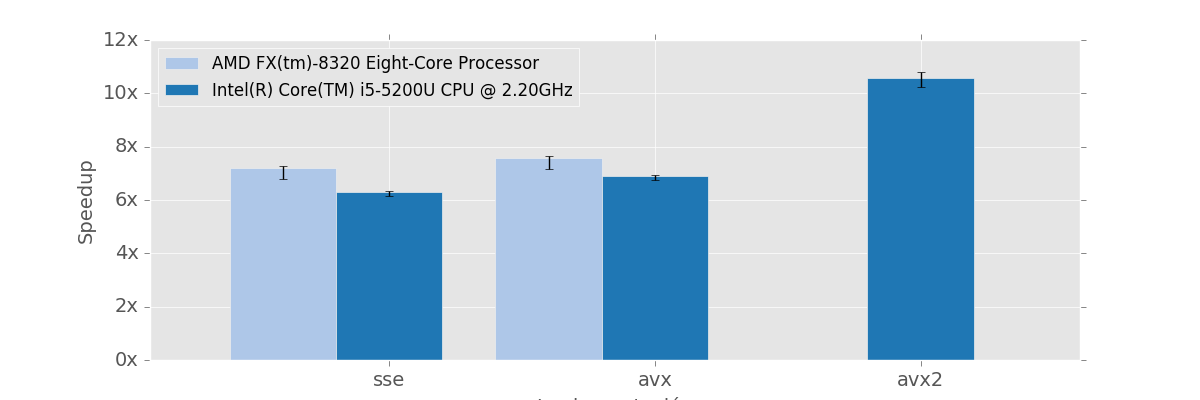
\includegraphics[width=\textwidth]{ldr-time-speedup}
    \caption{Speedup relativo respecto a la implementación en C compilada con O3 del filtro ldr sobre lena.bmp 512x512.}
    \label{fig:ldr-time-speedup}
\end{figure}

Encontramos una diferencia de performance muy grande entre la implementación de C y las implementaciones en assembler. Esto se puede deber a que el compilador de C no logra vectorizar el loop, como podemos ver en el dump de gdb.

\begin{lstlisting}
0x404662 <ldr_c+273>    movzx  ecx,BYTE PTR [rbp-0x8]
0x404666 <ldr_c+277>    add    eax,ecx
0x404668 <ldr_c+279>    movzx  ecx,BYTE PTR [rbp-0x2]
0x40466c <ldr_c+283>    add    eax,ecx
0x40466e <ldr_c+285>    movzx  ecx,BYTE PTR [rbp-0x3]
0x404672 <ldr_c+289>    add    eax,ecx
0x404674 <ldr_c+291>    movzx  ecx,BYTE PTR [rbp-0x4]
0x404678 <ldr_c+295>    add    eax,ecx
0x40467a <ldr_c+297>    movzx  ecx,BYTE PTR [rbp+0x2]
0x40467e <ldr_c+301>    add    eax,ecx
0x404680 <ldr_c+303>    movzx  ecx,BYTE PTR [rbp+0x1]
0x404684 <ldr_c+307>    add    eax,ecx
0x404686 <ldr_c+309>    movzx  ecx,BYTE PTR [rbp+0x0]
\end{lstlisting}

También vemos que el uso de instrucciones no destructivas de la extensión AVX y la operación de FMA logran un ligero aumento de performance, reduciendo el tiempo de ejecución en aproximadamente 10\% en los procesadores que probamos.

Por otro lado la implementación AVX2 corre un 50\% mas rápido que SSE, mostrando que los beneficios de procesar aún mas datos en paralelo sobrepasan el problema del aumento de la complejidad del código.

\subsubsection{Diferencias entre cálculos con enteros y con punto flotante}

\begin{figure}[H]
    \centering
    \begin{minipage}[t]{0.4\linewidth}
    \centering
    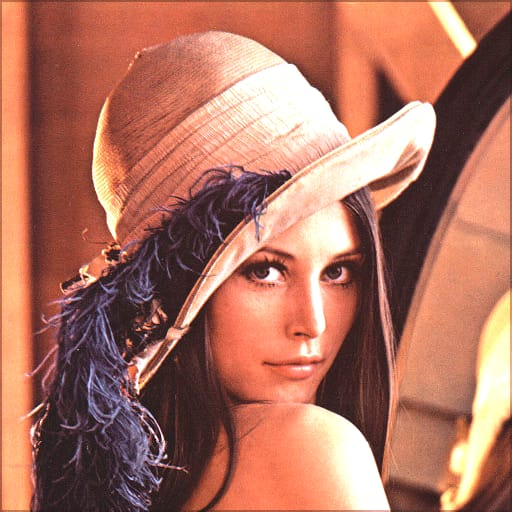
\includegraphics[width=\textwidth]{lena-ldr-c}
    Implementación de C
    \end{minipage}
    \hfill
    \begin{minipage}[t]{0.4\linewidth}
    \centering
    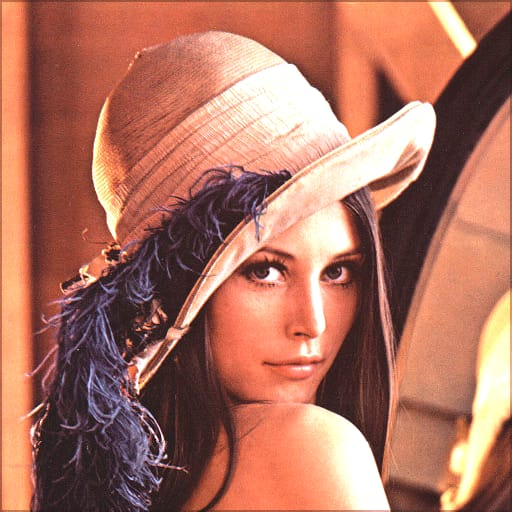
\includegraphics[width=\textwidth]{lena-ldr-c}
    Implementación SSE con punto flotante
    \end{minipage}
    \caption{Perdida de precisión en la implementación con cálculos de punto flotante. Ambas imágenes son ligeramente diferentes.}
    \label{fig:ldr-perdida-precision}
\end{figure}

Aún con el registro \asm{MXCSR} configurado para redondear siempre hacia cero al convertir números de punto flotante a enteros encontramos diferencias en las imágenes de salida. En una batería de imágenes de prueba encontramos que nunca un canal de un pixel difería en mas de 1 de la imágen original, y esta diferencia se encontraba en menos del 0.02\% de los píxeles.

\begin{figure}[H]
    \centering
    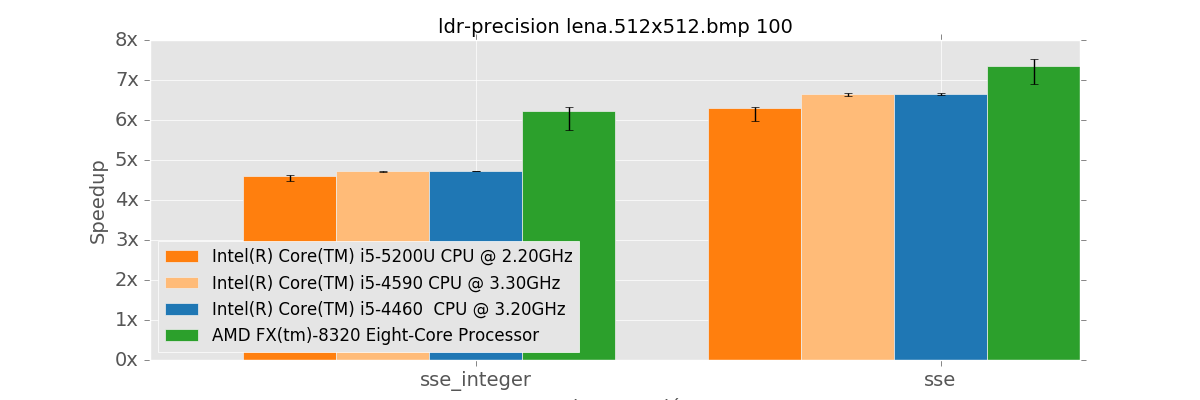
\includegraphics[width=\textwidth]{ldr-precision-time-speedup}
    \caption{Speedup relativo respecto a la implementación en C compilada con O3 del filtro ldr sobre lena.bmp 512x512.}
    \label{fig:ldr-precision-time-speedup}
\end{figure}

Considerando que la diferencia es tan mínima y que la implementación exacta usando calculos enteros resultó ser un 25\% mas lenta que la de punto flotante decidimos que para un uso general, tratandose de un filtro de imágenes que serán captadas por un ojo humano, resulta mucho mas conveniente usar cálculos de punto flotante.

\subsubsection{Throughput de píxeles en función del tamaño de imagen}

\begin{figure}[H]
    \centering
    \begin{minipage}[t]{0.49\linewidth}
    \centering
    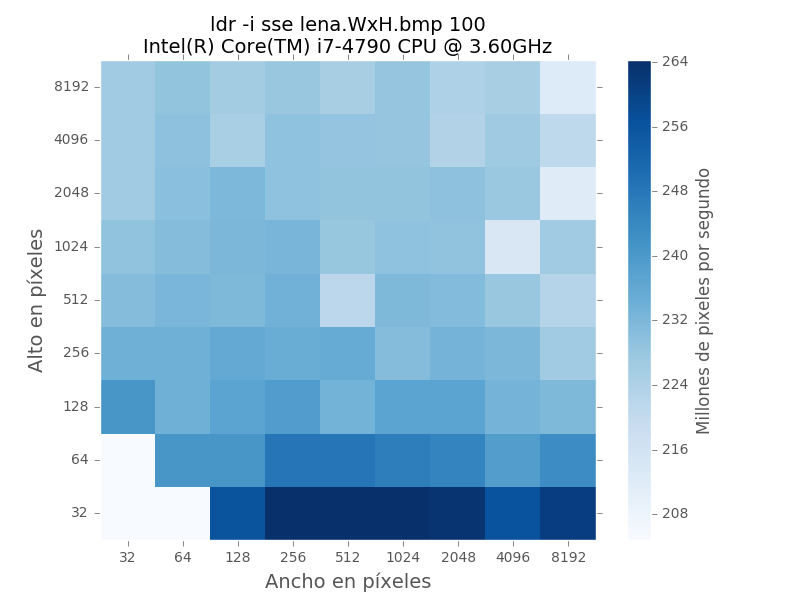
\includegraphics[width=\textwidth]{ldr-time-rel-map-sse-gflan-MS-7817}
    \end{minipage}
    \hfill
    \begin{minipage}[t]{0.49\linewidth}
    \centering
    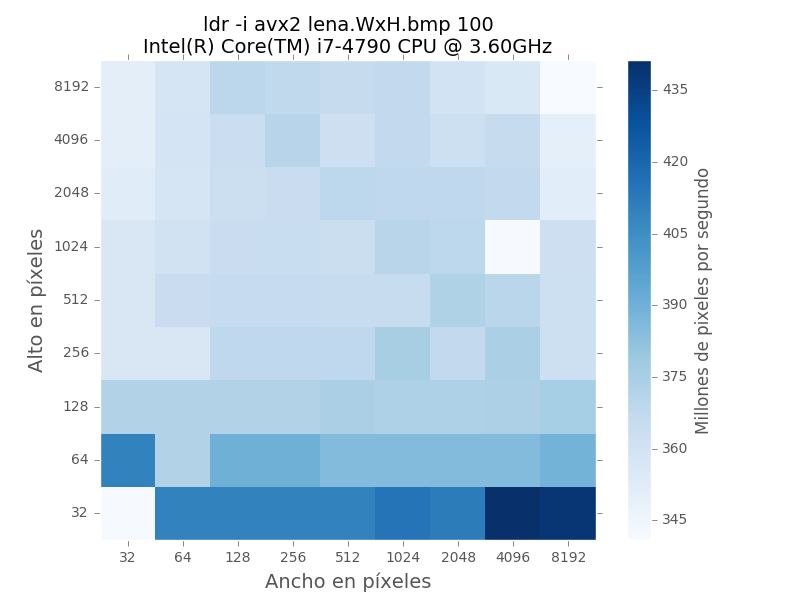
\includegraphics[width=\textwidth]{ldr-time-rel-map-avx2-gflan-MS-7817}
    \end{minipage}
    \caption{Millones de píxeles por segundo en implementación SSE y AVX2 en un procesador con 8MB de caché}
    \label{fig:ldr-perdida-precision}
\end{figure}

Observamos que el rendimiento se mantiene casi constante para la mayoría de los tamaños de imagen aún cuando el tamaño de la imagen sobrepasa el de la caché. Esto se debe a que el controlador de caché identifica perfectamente el patrón de accesos del algoritmo, y la cantidad de operaciones que se realizan en el ciclo le dan tiempo suficiente para prefetchear los datos necesarios de memoria.

Los valores se ven distorsionados cuando la imagen tiene poca altura ya que en ese caso la copia de las primeras y últimas dos filas, operacíon mucho mas rápida que los cálculos del filtro, representa un porcentaje mas alto de las operaciones. Como para la copia de los bordes se deben realizar accesos no secuenciales a memoria no vemos esta distorsión para imágenes con poco ancho.

